\chapter{Аналитический раздел}
В этом разделе будут проведена формализация задачи, рассмотрена методология вычислительных конвейеров и возможности для распараллеливания.

\section{Вычислительный конвейер}
Конвейер - система поточного производства \cite{mednov}.
Вычислительный конвейер — способ организации вычислений, используемый в современных процессорах и контроллерах с целью повышения их производительности,
а также технология, используемая при разработке компьютеров и других цифровых электронных устройств \cite{vliw}.

Идея заключается в параллельном выполнении нескольких инструкций процессора. 
Сложные инструкции процессора представляются в виде последовательности более простых стадий. 
Вместо выполнения инструкций последовательно (ожидания завершения конца одной инструкции и перехода к следующей), следующая инструкция может выполняться через несколько стадий выполнения первой инструкции. 
Это позволяет управляющим цепям процессора получать инструкции со скоростью самой медленной стадии обработки, однако при этом намного быстрее, чем при выполнении эксклюзивной полной обработки каждой инструкции от начала до конца.

На рисунке 1 представлен пример реализации вычислительного конвейера, где каждая буква означает одно из действий при выполнении процессором команды.
\FloatBarrier
\begin{figure}[h]
	\begin{center}
		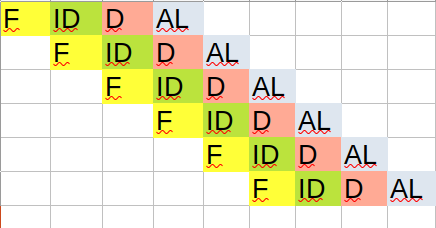
\includegraphics[]{inc/conv.png}
	\end{center}
	\caption{Демонстрация вычислительного конвейера}
\end{figure}
\FloatBarrier

\section{Основной алгоритм}
В качестве задачи для реализации выбрана следующая.
Пусть дан массив $ arr $. 
Требуется произвести стандартизацию данных.
Это означает, что каждый элемент массива должен быть преобразован по формуле 1.1:
\begin{equation}
{Arr}[i] = \frac{{Arr}[i] - \mu}{\sigma}
\end{equation}

где $\mu$ - среднее арифметическое массива, а $\sigma$ - стандартное отклонение.

\section{Реализация конвейера для основного алгоритма}
Выполнение задачи можно разбить на несколько этапов:
\begin{enumerate}
	\item Вычисление среднего арифметического массива.
	\item Вычисление дисперсии по элементам массива. Для этого требуется знать среднее арифметическое из первого этапа.
	\item Стандартизация по формуле 1.1 на основе дисперсии и среднего арифметического массива.
\end{enumerate}

Вычислительный конвейер может быть построен на этих трёх этапах, так как три задачи выполняются за один порядок времени, соответственно, конвейер не будет задерживаться на одном отрезке.

Каждый этап конвейера записывает результат в очередь следующего этапа, соответственно, требуется использовать мьютексы для того, чтобы исключить ошибки по памяти.

\section{Вывод}
Была рассмотрена методология вычислительного конвейера, произведена формализация задачи и рассмотрены способы распараллеливания основного алгоритма.